%=====================================================================
\section{Metodología}

\subsection{Proceso según CRISP-ML(Q)}
El estudio sigue el modelo de proceso CRISP-ML(Q) \cite{Studer2021}, que organiza el desarrollo en seis etapas con controles de calidad: comprensión del negocio y de los datos, preparación de los datos, modelado, evaluación, despliegue, y monitoreo y mantenimiento. Este artículo documenta las etapas 1 a 4 y discute las etapas 5 y 6 como viabilidad. Este entregable cubre la comprensión de los datos (etapa 2) y la elección de los modelos (inicio de la etapa 3).

\subsection{Conjunto de datos}
El historial de \texttt{torvalds/linux} permite responder la pregunta porque trae, en el mismo registro, la información disponible al integrar cada commit (diff, trailers y fechas) y la etiqueta posterior (el \texttt{Fixes:} que lo señala), y porque cubre sin cortes el año 2026, en el que se mide la degradación. Con el kernel trabajaron también Lyu \emph{et al.} \cite{Lyu2024}, que validan la etiqueta \texttt{Fixes:} frente a SZZ, y Nguyen \emph{et al.} \cite{Nguyen2025}, que reportan AUC-PR con la prevalencia real, lo que permite comparar órdenes de magnitud. El conjunto de Zenodo de Maes Bermejo \emph{et al.} \cite{MaesBermejo2024} termina en noviembre de 2023, así que no cubre la validación de 2024--2025 ni la prueba, y se usó solo para contrastar la etiqueta. Por eso se minó el clon completo.

Se recorrió la rama principal con una sola pasada de \texttt{git log}, sin commits de fusión, desde 2014; los años 2014--2018 solo alimentan la experiencia de los autores. Las referencias \texttt{Fixes:} (prefijos de al menos 8 caracteres hexadecimales) se resuelven contra el historial: el 9,4\,\% que no se resuelve apunta a commits anteriores a 2014 o a otros árboles. Un commit es \emph{riesgoso} si un commit posterior de la rama principal lo cita con \texttt{Fixes:} en 90 días o menos. Los commits con menos de 90 días de observación a la fecha de corte quedan \emph{censurados} y se excluyen (\cifCensurados{} commits), porque su etiqueta negativa todavía no es definitiva \cite{Falessi2022,Cabral2019}. La Tabla~\ref{tab:ficha} resume la ficha del conjunto, elaborada según la propuesta \emph{Datasheets for Datasets} \cite{Gebru2021}.

\begin{table}[!t]
\caption{Ficha del conjunto de datos}
\label{tab:ficha}
\centering\footnotesize
\begin{tabularx}{\columnwidth}{@{}p{2.2cm} Y@{}}
\toprule
\cabecera \textbf{Campo} & \textbf{Descripción}\\
\midrule
Nombre y versión & Commits de \texttt{torvalds/linux}, rama \texttt{master}; clon del 2026-11-07\\
Fuente y enlace & \url{https://github.com/torvalds/linux}; minado con \texttt{src/minar\_kernel.py}\\
Licencia & Código GPL-2.0; metadatos de git públicos\\
Contexto & Commits integrados por los mantenedores; fechas de autor y de committer\\
Tamaño & \cifCommits{} commits no censurados $\times$ \cifNVariables{} variables de entrada; eventos irregulares, 2019-01-01 a 2026-07-31\\
Variable objetivo & \texttt{riesgoso} (0/1): citado por un \texttt{Fixes:} en $\le$90 días. Clasificación binaria\\
Variables de entrada & Tamaño, difusión, revisión, propósito, experiencia y momento; diccionario con unidades en la Tabla~A1 del anexo\\
Faltantes y atípicos & 0\,\% de faltantes en todas las variables. Atípicos: colas pesadas reales (hasta 730.092 líneas en un commit); se conservan y se tratan con transformaciones por rangos\\
Sesgos conocidos & Solo se ven los defectos que alguien corrigió con \texttt{Fixes:}; la adopción del trailer crece hasta 2019; \texttt{drivers/} concentra el 49\,\% de los commits y el 1\,\% de los autores, el 39\,\%\\
Uso previsto & Priorizar la revisión de commits. No se recomienda para evaluar personas: los autores están anonimizados con SHA-256 con sal\\
\bottomrule
\end{tabularx}
\end{table}

\subsection{Verificación de los criterios de calidad D1--D7}
La Tabla~\ref{tab:d1d7} verifica los siete criterios mínimos de validación del conjunto con la evidencia cuantitativa de cada uno. Todas las cifras se calculan con el conjunto de desarrollo (2019--2025); de la prueba solo se cuenta su tamaño.

\begin{table}[!t]
\caption{Verificación de los criterios D1--D7}
\label{tab:d1d7}
\centering\footnotesize
\begin{tabularx}{\columnwidth}{@{}p{1.8cm} Y p{0.95cm}@{}}
\toprule
\cabecera \textbf{Criterio} & \textbf{Evidencia} & \textbf{¿Cumple?}\\
\midrule
D1 Tamaño ($\ge$300 obs.) & $n$ = \cifCommits{}: \cifDesarrollo{} de desarrollo y \cifPrueba{} de prueba & Sí\\
D2 Objetivo definido & \texttt{Fixes:} en $\le$90 días con censura de 90 días; \cifPositivosDesarrollo{} positivos en desarrollo (\cifPrevMin{}--\cifPrevMax{} por año) & Sí\\
D3 Calidad & 0\,\% de faltantes en el objetivo y en las entradas; 0 hashes duplicados. \cifParesCherry{} pares del mismo parche por \emph{cherry-pick} entre árboles (\cifFracCherry{} del desarrollo), \cifDiscCherry{} con etiqueta distinta; los backports a \emph{stable} no están en la rama principal & Sí\\
D4 Estructura & Ordenado por fecha del committer (la de integración); eventos irregulares; \cifAutores{} autores y \cifSubsistemas{} subsistemas como grupos & Sí\\
D5 Disponibilidad & Solo el propio commit y los commits anteriores del autor; ninguna variable descartada por fuga & Sí\\
D6 Licencia y ética & GPL-2.0; nombres y correos reemplazados por SHA-256 con sal; no se publican los mensajes & Sí\\
D7 Documentación & Diccionario con origen y unidad de las \cifNVariables{} variables (Tabla~A1); fecha del clon en la ficha & Sí\\
\bottomrule
\end{tabularx}
\end{table}

\textbf{Revisión de los \emph{cherry-picks} (D3).} Se buscó en los mensajes la marca \emph{``cherry picked from commit''} y se comprobó si el commit original también está en la rama principal (\texttt{src/e2\_backports.py}). Casi todos los pares tocan \texttt{drivers/gpu/drm}, cuyos árboles llevan una corrección a \emph{-fixes} y la dejan también en \emph{-next}. Las dos copias distan una mediana de \cifDiasCherry{} días, así que casi siempre caen en el mismo bloque temporal, y las \cifDiscCherry{} etiquetas discordantes son una fracción mínima del desarrollo, por debajo del ruido de la propia etiqueta (81\,\% de culpables confirmados \cite{Lyu2024}). Se conservan ambas copias y se declara como excepción justificada.

\subsection{Análisis exploratorio}
Antes de explorar se reservó el bloque de prueba: los commits del 1 de enero al 31 de julio de 2026. Toda la exploración usa solo el conjunto de desarrollo (2019--2025), y de la prueba no se miró ni la etiqueta ni la distribución de las entradas.

La Tabla~\ref{tab:desc} presenta los estadísticos descriptivos de las diez variables del modelo difuso; las \cifNVariables{} están en el anexo. Las variables de tamaño tienen colas extremas: la media de líneas añadidas es de unas 59, pero el máximo pasa de 730.000 y la desviación estándar es 27 veces la media. La experiencia del autor también es muy asimétrica, por unos pocos mantenedores con miles de commits.

\begin{table}[!t]
\caption{Estadísticos descriptivos (conjunto de desarrollo, 2019--2025)}
\label{tab:desc}
\centering\scriptsize
\setlength{\tabcolsep}{3pt}
\begin{tabular}{@{}l l r r r r r@{}}
\toprule
\cabecera \textbf{Variable} & \textbf{Unidad} & \textbf{Media} & \textbf{DE} & \textbf{Mín.} & \textbf{Máx.} & \textbf{\%\,falt.}\\
\midrule
\texttt{riesgoso} & 0/1 & \multicolumn{4}{l}{prevalencia anual \cifPrevMin{}--\cifPrevMax{}} & 0{,}0\\
\filas{../comun/tabla_descriptivos.tex}
\bottomrule
\end{tabular}
\end{table}

La Fig.~\ref{fig:objetivo} muestra la distribución de la variable objetivo y su relación con el tamaño, y la Fig.~\ref{fig:corr} la matriz de correlación de Spearman entre las entradas. Se usa Spearman y no Pearson porque las colas pesadas harían que unos pocos commits enormes dominaran el coeficiente.

\begin{figure}[!t]
\centering
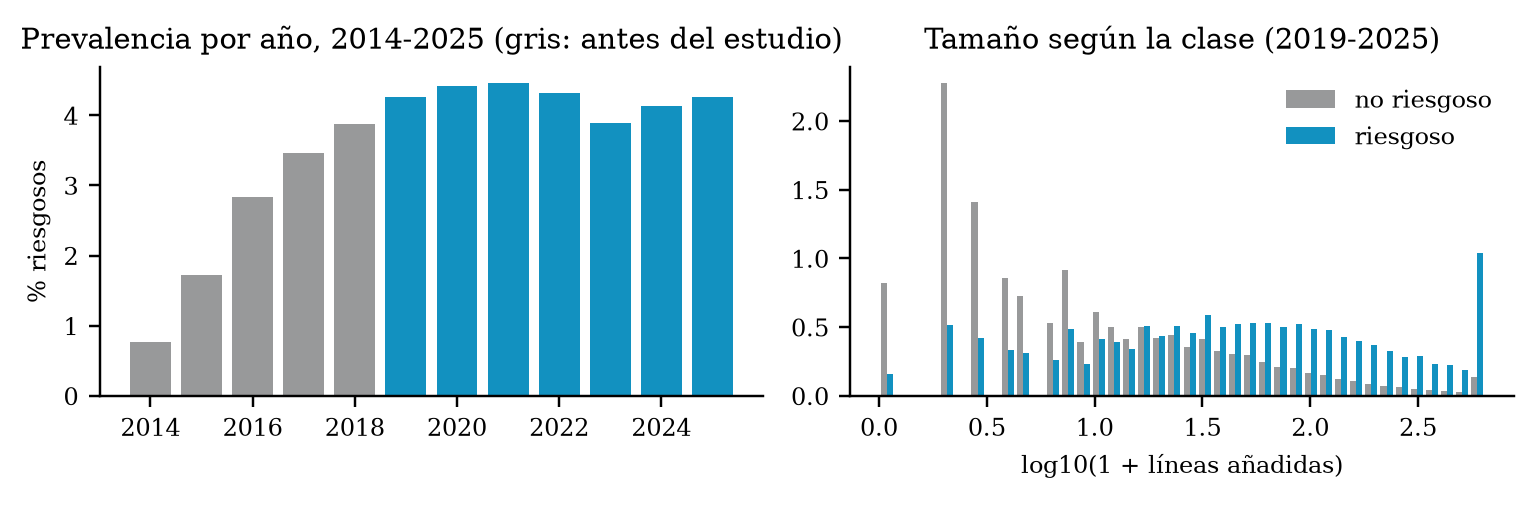
\includegraphics[width=\columnwidth]{../../resultados/e2/prevalencia_y_tamano.png}
\caption{Variable objetivo. Izquierda: balance de clases (prevalencia de riesgosos) por año, 2014--2025; en gris, los años anteriores al estudio. Derecha: distribución de las líneas añadidas por clase en el desarrollo.}
\label{fig:objetivo}
\end{figure}

\begin{figure}[!t]
\centering
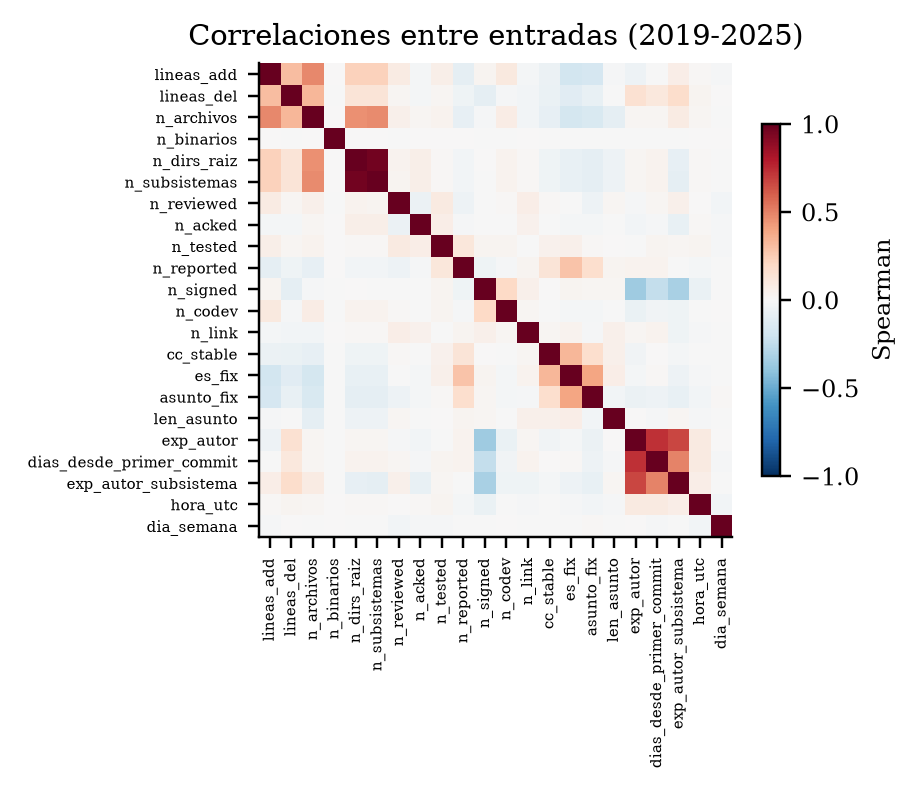
\includegraphics[width=0.92\columnwidth]{../../resultados/e2/correlaciones.png}
\caption{Matriz de correlación de Spearman entre las \cifNVariables{} variables de entrada (desarrollo, 2019--2025).}
\label{fig:corr}
\end{figure}

Los hallazgos del análisis exploratorio orientan las decisiones de preparación y modelado:
\begin{itemize}
\item \textbf{La prevalencia crece hasta 2018 por la adopción de \texttt{Fixes:}} y desde 2019 se estabiliza entre \cifPrevMin{} y \cifPrevMax{} $\rightarrow$ el entrenamiento empieza el 1 de enero de 2019.
\item \textbf{Clases desbalanceadas} (cerca del 4\,\% de positivos) $\rightarrow$ la métrica principal es el AUC-PR \cite{Saito2015} y no se remuestrea, para que la prevalencia de validación sea la real.
\item \textbf{El tamaño es la señal dominante y no es lineal}: la prevalencia pasa de \cifPrevQunoAdd{} en el quintil más pequeño de líneas añadidas a \cifPrevQcincoAdd{} en el más grande, con colas extremas $\rightarrow$ el modelo difuso trabaja sobre la función de distribución empírica y la regresión logística sobre $\log(1+x)$ estandarizado, ambos ajustados solo con el entrenamiento.
\item \textbf{Dos pares casi redundantes}: directorios de primer nivel y subsistemas ($\rho$ = 0,97), y experiencia y antigüedad del autor ($\rho$ = 0,73) $\rightarrow$ el modelo difuso usa solo uno de cada par.
\item \textbf{Deriva en las covariables antes de 2026}: los \texttt{Reviewed-by} por commit suben de \cifReviewedIni{} (2019) a \cifReviewedFin{} (2025) y las correcciones, de \cifFixIni{} a \cifFixFin{} $\rightarrow$ validación por ventanas temporales y no validación cruzada aleatoria.
\end{itemize}

\subsection{Modelos del estudio}
La Tabla~\ref{tab:modelos} define los modelos del estudio y el papel de cada uno. Los modelos se fijaron antes de observar el conjunto de prueba. La regresión logística es el estándar de JIT y es difícil de superar con partición temporal \cite{Kamei2013,Zeng2021}; el \emph{gradient boosting} \cite{Friedman2001} da la cota alta de una caja negra sobre las mismas variables.

\begin{table}[!t]
\caption{Modelos del estudio y su papel}
\label{tab:modelos}
\centering\footnotesize
\begin{tabularx}{\columnwidth}{@{}p{1.35cm} p{1.5cm} Y p{1.15cm}@{}}
\toprule
\cabecera \textbf{Papel} & \textbf{Modelo} & \textbf{Justificación} & \textbf{Parám.}\\
\midrule
Referencia trivial & Clase mayoritaria & Su AUC-PR es la prevalencia: fija el piso & 0\\
Referencia clásica & Regresión logística & Estándar de JIT \cite{Kamei2013,Zeng2021} & 23\\
Referencia clásica fuerte & \emph{Gradient boosting} & Cota alta sin restricción de interpretabilidad \cite{Friedman2001} & $\le$12.600 hojas\\
Propuesto & Difuso-evolutivo & $\le$15 reglas legibles; vértices y reglas ajustados con un AG \cite{Herrera2008,Ishibuchi2001} & \cifGenes{} genes (\cifGenesReales{} reales)\\
Variante sin evolución & Difuso voraz & Mismas reglas iniciales, sin AG: aísla el aporte de la evolución & $\le$15 pesos\\
\bottomrule
\end{tabularx}
\end{table}

Cada variable $x_j$ se lleva a $z_j\in[0,1]$ con su función de distribución empírica, estimada solo con el entrenamiento. Sobre $z_j$ se definen tres términos (bajo, medio y alto) que forman una partición de Ruspini \cite{Ruspini1969} con vértices $a_j<b_j<c_j$. El modelo propuesto se formula como
\begin{equation}
\mu_r(\mathbf{x})=\prod_{(j,t)\in A_r}\mu_{jt}(z_j),\qquad
\hat{y}=s(\mathbf{x})=1-\prod_{r=1}^{R}\bigl(1-w_r\,\mu_r(\mathbf{x})\bigr),
\end{equation}
donde $A_r$ es el conjunto de hasta tres antecedentes (variable $j$, término $t$) de la regla $r$, $\mu_{jt}$ la pertenencia de $z_j$ al término $t$, $w_r\in[0,1]$ el peso de la regla, $R\le15$ el número de reglas activas y $s(\mathbf{x})$ el puntaje de riesgo que ordena los commits (t-norma producto y O probabilístico entre reglas).

El ajuste sigue el enfoque Pittsburgh \cite{Herrera2008,Ishibuchi2001}: cada individuo codifica los $3\times10$ vértices y la base completa de 15 reglas (activación, hasta tres pares variable--término y peso), \cifGenes{} genes en total. La aptitud es el AUC-PR de entrenamiento menos $\lambda$ por antecedente. Los operadores son selección por torneo de 3 con elitismo de 2, cruce uniforme que hereda cada regla completa, y mutación gaussiana de vértices y pesos y aleatoria de antecedentes y términos. El espacio de búsqueda es: población $\{40, 60, 80\}$, generaciones $\{60, 100, 140\}$, reglas $\{5, 10, 15\}$, probabilidad de mutación $\{0{,}05; 0{,}15; 0{,}3\}$, de cruce $\{0{,}7; 0{,}9\}$ y $\lambda\in\{0; 0{,}0005\}$. La variante sin evolución fija los vértices en los cuantiles $(0{,}2; 0{,}5; 0{,}8)$ y elige reglas de 1 o 2 antecedentes de forma voraz; esa misma solución siembra un cuarto de la población inicial del AG.

\textbf{(i) Propiedad de los datos que aprovecha.} El riesgo crece por umbrales con el tamaño y la difusión y se modula con la revisión y la experiencia. Una partición difusa sobre la escala de cuantiles captura esos umbrales sin depender de las colas, y las reglas cortas expresan interacciones que un mantenedor reconoce, como ``si el cambio es grande y toca varios subsistemas''.

\textbf{(ii) Mejores modelos de la matriz y por qué este.} En la matriz, los mejores AUC son de redes profundas y modelos preentrenados sobre el diff \cite{Ni2022}, pero con partición temporal una regresión logística las iguala \cite{Zeng2021}, y ninguno es legible. Se elige un clasificador difuso-evolutivo porque es el vacío identificado y porque el criterio de éxito exige interpretabilidad.

\textbf{(iii) Número de parámetros frente al tamaño.} El individuo tiene \cifGenes{} genes, de los que \cifGenesReales{} son reales. La aptitud se calcula sobre \cifFilasAptitud{} commits (de unos 300.000 en la primera ventana de entrenamiento), más de 500 por gen, así que el riesgo de sobreajuste es bajo; el límite de 15 reglas responde a la interpretabilidad y no al tamaño. La regresión logística (23 parámetros) y el \emph{gradient boosting} (hasta 200 árboles de 63 hojas) también quedan muy por debajo del tamaño del conjunto.

\textbf{(iv) Presupuesto de cómputo.} Cada entrenamiento evalúa hasta \cifEvalAptitud{} individuos (población $\times$ generaciones) sobre una muestra fija de \cifFilasAptitud{} commits. La configuración más cara tardó \cifSegEntrenamiento{} s en un Apple M1 (8 núcleos, 8 GB). El plan prevé \cifNEntrenamientos{} entrenamientos: 14 configuraciones de la búsqueda aleatoria, 9 de sensibilidad y 5 semillas, cada uno en 3 ventanas. Eso suma como cota superior \cifHorasCota{} h en un núcleo, que caben en el presupuesto de una noche y se reducen al paralelizar.

\subsection{Partición prevista y métrica principal}
La partición es por bloques temporales con un hueco de 90 días: para cada año de validación (2023, 2024 y 2025) se entrena desde 2019 hasta 90 días antes de su inicio, y la prueba es enero--julio de 2026, que se evalúa una sola vez. La métrica principal es el AUC-PR, con la que se juzga el criterio de éxito de la Tabla~\ref{tab:criterio}. El preprocesamiento sin fuga se desarrolla en el Entregable 3.
